%% -*- coding:utf-8 -*-
\chapter{Objects and morphisms}

\section{Equality}

The important question is how can we decide whenever an
object/morphism is equal to another object/morphism? The trivial
answer is possible for if an \mynameref{def:object} is a
\mynameref{def:set}. In this case we can say that 2 objects are equal
if they contains the same elements. Unfortunately we cannot do the
same for default objects as soon as they don't have any internal
structure. We can use the same trick as in
\mynameref{rem:set_vs_category}: if we cannot use ``microscope'' lets
use ``telescope'' and define the equality of objects and morphisms of
a category $\cat{C}$ in the terms of whole $\cathom{C}$.

\begin{definition}[Objects equality]
\label{def:object_equality}
Two \mynameref{def:object}s $a$ and $b$ in \mynameref{def:category}
$C$ are equal if there exists an unique \mynameref{def:isomorphism}
$f: a \to b$. This also means that also exist unique isomorphism $g: b
\to a$. These two \mynameref{def:morphism}s are related each other via
the following equations: $f \circ g = \idarrow[a]$ and $g \circ f
= \idarrow[b]$. 
\end{definition}

Unlike \mynameref{def:function}s between \mynameref{def:set}s we don't
have any additional info 
\footnote{
for instance info about sets internals. i.e. which elements of the sets
are connected by the considered functions
}
about \mynameref{def:morphism}s except
category theory axioms which the morphisms satisfied
\cite{bib:stackexchange:morphism:equality}. This leads us to the
following definition for morphims equality:
\begin{definition}[Morphisms equality]
\label{def:morphism_equality}
Two \mynameref{def:morphism}s $f$ and $g$ in \mynameref{def:category}
$C$ are equal if the equality can be derived from the base axioms: 
\begin{itemize}
\item \mynameref{axm:composition}
\item \mynameref{axm:associativity}
\item \mynameref{def:id}: \eqref{eq:leftid}, \eqref{eq:rightid}
\end{itemize}
or \mynameref{def:commutative_diagram}s which postulate the equality.
\end{definition}

As an example lets proof the following theorem
\begin{theorem}[Identity is unique]
\label{thm:identity_unique}
The \mynameref{def:id} is unique.
\begin{proof}
Consider an \mynameref{def:object} $a$ and it's \mynameref{def:id} 
$\idarrow[a]$. Let $\exists f: a \to a$ such that $f$ is also
identity. In the case \eqref{eq:leftid} for $f$ as identity gives
\[
f \circ \idarrow[a] = \idarrow[a].
\]
From other side \eqref{eq:rightid} for $\idarrow[a]$ satisfied
\[
f \circ \idarrow[a] = f
\]
i.e. $f = \idarrow[a]$.
\end{proof}
\end{theorem}

\section{Initial and terminal objects}
\begin{definition}[Initial object]
\label{def:initial_object}
Let $\cat{C}$ is a \mynameref{def:category}, the
\mynameref{def:object} $i \in \catob{C}$ is called
\textit{initial object} if $\forall x \in \catob{C}
\exists! f_x: i \to x \in \cathom{C}$.
\end{definition}

\begin{definition}[Terminal object]
\label{def:terminal_object}
Let $\cat{C}$ is a \mynameref{def:category}, the
\mynameref{def:object} $t \in \catob{C}$ is called
\textit{terminal object} if $\forall x \in \catob{C}
\exists! g_x: x \to t \in \cathom{C}$.
\end{definition}

As you can see the initial and terminal objects are opposite each
other. I.e. if $i$ is an \mynameref{def:initial_object} in $\cat{C}$
then it will be \mynameref{def:terminal_object} in
the \mynameref{def:op_category} $\cat{C^{op}}$.

\begin{theorem}[Initial object is unique]
\label{thm:initial_object_unique}
Let $\cat{C}$ is a category and $i, i' \in \catob{C}$ two
\mynameref{def:initial_object}s then there exists an unique
\mynameref{def:isomorphism} $u: i \to i'$ (see
\mynameref{def:object_equality}) 
\begin{proof}
Consider the following \mynameref{def:commutative_diagram} (see
\cref{fig:initial_object_unique}) 
\begin{figure}
  \centering
  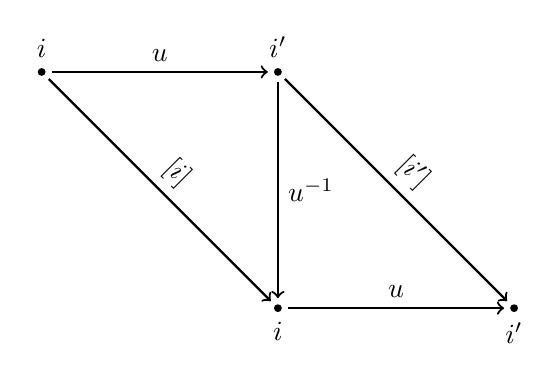
\begin{tikzpicture}[ele/.style={fill=black,circle,minimum
        width=.8pt,inner sep=1pt},every fit/.style={ellipse,draw,inner
        sep=-2pt}]

    % the texts
    
    \node[ele,label=above:$i$] (i1) at (0,3) {};    
    \node[ele,label=above:$i'$] (i2) at (3,3) {};    
    \node[ele,label=below:$i$] (i12) at (3,0) {};
    \node[ele,label=below:$i'$] (i22) at (6,0) {};

    \draw[->,thick,shorten <=2pt,shorten >=2pt] (i1) to
    node[sloped,above]{$u$} (i2);
    \draw[->,thick,shorten <=2pt,shorten >=2] (i12) to
    node[sloped,above]{$u$} (i22); 
    \draw[->,thick,shorten <=2pt,shorten >=2] (i1) to
    node[sloped,above]{$\idarrow[i]$} (i12); 
    \draw[->,thick,shorten <=2pt,shorten >=2] (i2) to
    node[sloped,above]{$\idarrow[i']$} (i22); 
    \draw[->,thick,shorten <=2pt,shorten >=2] (i2) to
    node[right]{$u^{-1}$} (i12); 
  \end{tikzpicture}
  \caption{Commutative diagram for initial object unique proof}
  \label{fig:initial_object_unique}
\end{figure}
\end{proof}
\end{theorem}

\begin{theorem}[Terminal object is unique]
\label{thm:terminal_object_unique}
Let $\cat{C}$ is a category and $t, t' \in \catob{C}$ two
\mynameref{def:terminal_object}s then there exists an unique
\mynameref{def:isomorphism} $v: t' \to t$ (see
\mynameref{def:object_equality}) 
\begin{proof}
Just got to the \mynameref{def:op_category} and revert arrows in
\cref{fig:initial_object_unique}. The result shown on
\cref{fig:terminal_object_unique} and it proofs the theorem statement.
\begin{figure}
  \centering
  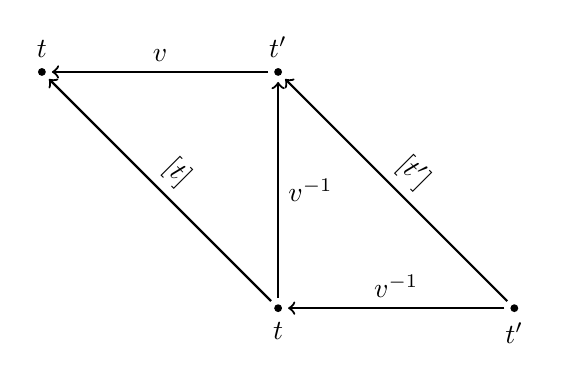
\begin{tikzpicture}[ele/.style={fill=black,circle,minimum
        width=.8pt,inner sep=1pt},every fit/.style={ellipse,draw,inner
        sep=-2pt}]

    % the texts
    
    \node[ele,label=above:$t$] (t1) at (0,3) {};    
    \node[ele,label=above:$t'$] (t2) at (3,3) {};    
    \node[ele,label=below:$t$] (t12) at (3,0) {};
    \node[ele,label=below:$t'$] (t22) at (6,0) {};

    \draw[->,thick,shorten <=2pt,shorten >=2pt] (t2) to
    node[sloped,above]{$v$} (t1);
    \draw[->,thick,shorten <=2pt,shorten >=2] (t22) to
    node[sloped,above]{$v^{-1}$} (t12); 
    \draw[->,thick,shorten <=2pt,shorten >=2] (t12) to
    node[sloped,above]{$\idarrow[t]$} (t1); 
    \draw[->,thick,shorten <=2pt,shorten >=2] (t22) to
    node[sloped,above]{$\idarrow[t']$} (t2); 
    \draw[->,thick,shorten <=2pt,shorten >=2] (t12) to
    node[right]{$v^{-1}$} (t2); 
  \end{tikzpicture}
  \caption{Commutative diagram for terminal object unique proof}
  \label{fig:terminal_object_unique}
\end{figure}
\end{proof}
\end{theorem}


\section{Product and sum}
TBD

\section{Examples}

\subsection{\textbf{Set} category}
\begin{example}[Initial object][\textbf{Set}]
\label{ex:set_initial_object}
Note that there is only one function from empty set to any other sets
\cite{bib:proofwiki:Empty_Mapping_is_Unique} that makes the empty set
as the \mynameref{def:initial_object} in \mynameref{ex:setcategory}. 
\end{example}

\begin{example}[Terminal object][\textbf{Set}]
\label{ex:set_terminal_object}
\mynameref{def:terminal_object} in \mynameref{ex:setcategory} is a set
with one element. 
\end{example}


\subsection{Programming languages}
\subsubsection{\textbf{Hask} category}
\begin{example}[Initial object][\textbf{Hask}]
\label{ex:hask_initial_object}
\mynameref{def:initial_object} in \mynameref{ex:haskcategory} is an
type without values 
\begin{minted}{haskell}
data Empty
\end{minted}
i.e. you cannot construct a object of the type.
\end{example}

\begin{example}[Terminal object][\textbf{Hask}]
\label{ex:hask_terminal_object}
Terminal object (unit) in mynameref{ex:haskcategory} keeps only one element
\begin{minted}{haskell}
data () = ()
\end{minted}
i.e. you can create only one element of the type.
\end{example}

TBD
\subsubsection{\textbf{C++} category}
TBD
\subsubsection{\textbf{Scala} category}
TBD

\subsection{Quantum mechanics}
TBD

